\documentclass{article}
\usepackage{authblk}
\usepackage[T1]{fontenc}
\usepackage[utf8]{inputenc}
\usepackage{graphicx}

\title{Recursion, Game Trees and Classes - Making an unbeatable algorithm.}

\author[]{Tushar Rakheja}
\author[]{Shibjash Dutt}
\author[]{Hanit Banga}

\affil[]{\texttt{Instructors @ Endofline Computer Club}}

\renewcommand\Authands{ and }

\date{August 2015}

\begin{document}

\maketitle

\section{Introduction}

In the last session, we talked about functions. We'll start this session by talking about recursive functions. These are functions that refer to themselves, in order to compute what they're meant to. We'll discuss the theory, some classic examples, and some interesting questions that are recursive in nature. \\

\noindent After that, we'll take a slight detour into programming and learn about lists in Python. A list is a data structure \cite{DSinPres_Slide} that stores elements sequentially.\\

\noindent Once we're done with lists, we'll come back to Tic-Tac-Toe, but this time we'll look at it with little to no code. We'll then introduce the tree data structure, and the class programming construct. Finally, we'll put all of it together, and assemble the Earth's Mightiest Zeros. 

\section{Recursive Functions}

\section{Lists}

\section{Trees}

\section{Game States} 

So far, we've looked at various tools, like functions, recursion and lists,
which will help us in our analysis of the game. Let us now start working with
a more concrete idea, that of \textit{game states}. \\

\noindent Imagine a game of Tic-Tac-Toe played between Alice and Bob. Alice is playing crosses (X) and Bob is playing zeros (O). \\

\noindent Here is an example of how such a game might proceed, if Alice plays first:

\begin{center}
    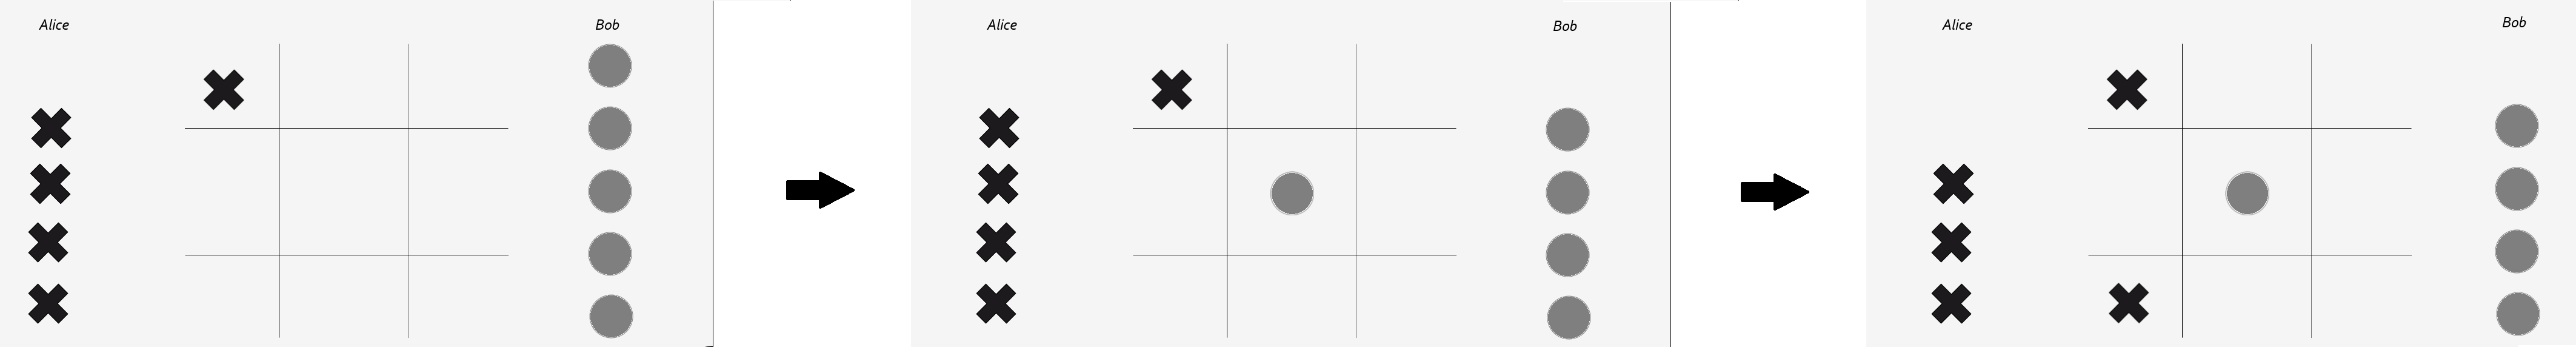
\includegraphics[scale=0.11]{AliceVBob}
\end{center}

\noindent And so on.

\section{Classes}

\section{Putting it all together}

\subsection{Game Trees}

\subsection{Relation between Game Trees and a Game State}



\begin{thebibliography}{9}
\bibitem{DSinPres_Slide}
Tushar Rakheja and Shibjash Dutt.
\textit{"CS. What it is, what it isn't, and why you should care."}
\texttt{https://github.com/EndoflineComputerClub/TicTacTongue.}
\\PresentationCS.pptx, slide 11. 
\end{thebibliography}

\end{document}